
\titlespacing*{\paragraph}{0pt}{0.4ex}{0.2ex}

\makeatletter
\titleformat{\chapter}[block]
  {\normalfont\huge\bfseries\color{ImperialBlue}}
  {\thechapter}{20pt}{\huge}
\titlespacing*{\chapter}{0pt}{-20pt}{15pt}
\makeatother

\chapter{Introduction}
\label{ch1}

\begin{spacing}{0.3}
\minitoc
\end{spacing}

\thesisspacing

\section{Project Overview}

The goal of this project was to design and implement a real-time 3D graphics
engine on the Xilinx PYNQ-Z1 SoC FPGA, using ray marching with signed
distance functions (SDFs), mounted inside a VR headset so that head orientation
controls the camera viewpoint live.

Ray marching was selected because it is embarrassingly parallel: each pixel's
colour is determined by tracing a single ray and evaluating an SDF at
successive steps. No pixel depends on any other, so every pixel can be computed
in a fully independent, deeply pipelined hardware path. By replacing the
marched vector coordinates with those of a canonical cell, space repetition is
enabled, allowing infinite psychedelic scenes and Mandel fractal sets in 3D.

\paragraph{Hardware accelerator: }
 The PL implements the rendering engine in SystemVerilog, built from a custom
27-bit floating-point library covering addition, subtraction, multiplication,
division, inverse square root, length, modulus, floor, and matrix--vector
products. Two independent \texttt{march\_core} instances run in parallel, each
fed by a round-robin pixel dispatcher. Completed pixels are burst to DDR3 via
AXI4, and an AXI VDMA IP outputs \(1024 \times 600\) pixels over HDMI at
74.25\,MHz. The system runs at 125\,MHz, achieving 18--40\,fps depending on
scene complexity. Camera and SDF parameters are transferred from the ARM
Cortex-A9 to the PL via an AXI-Lite register file at \texttt{0x43C00000}.

\paragraph{Software and user interface: }
 The PS runs Python on the PYNQ Linux stack. A graphical scene selector is
rendered into a VDMA framebuffer, allowing the user to choose from nine SDF
scenes via three push-buttons, triggering a runtime bitstream swap via PYNQ's
\texttt{Overlay} API.

\paragraph{IMU and VR headset: }
 An MPU-6050 IMU over I\textsuperscript{2}C provides pitch, roll, and yaw,
fused via a complementary filter to construct the camera lookat matrix each
frame.

\paragraph{Music reactivity: } 
 A 1024-point FFT is computed on loopback audio at 44.1\,kHz on the host PC.
Bass, mid, and treble energy bands, RMS, spectral centroid, and a beat
detection flag are streamed over TCP and written to AXI-Lite SDF parameter
registers, directly modulating geometry and camera path in real time.

\paragraph{Neural SDF (future work): }
A 4-layer MLP (3--32--32--32--1) in Q4.12 fixed-point was designed, with
\texttt{sdf\_nn.sv} and a trilinear interpolation cache implemented, but full
integration was not completed and is left as a future extension.

\paragraph{Scenes demonstrated: }
Nine SDF scenes are demonstrated: Scaffold, Sphere, Twisted Torus, Gyroid,
Hyperboloid, Octahedron, Star, Torus, and Mandelbox, all selectable at runtime.

% Team Roles and Responsibilities + Gantt Chart
% Requires in preamble: \usepackage{pgfgantt} \usepackage{booktabs} \usepackage{array}
% \input{team_roles}

\subsection{Team Roles and Responsibilities}
It was decided to split work between strengths of different members; EIE members would do the Vivado plumbing, debug, addressing of memory, AXI tooling and development of the hardware stack; and EEE members would focus on baseline RTL: Verilog modules, leaving Hardware Software Co Design to EIE students having done Information Processing.
It was decided to divide ownership of the system by subsystem, with each member
responsible for design and implementation of their area. Testing was done by other members to systematically cross verify work.
Extensive work has been deployed for code readability through comments on every module.
Table~\ref{tab:team_roles} gives a high-level summary; the subsections below
expand on each member's contribution.

{\renewcommand{\arraystretch}{2.0}
\begin{table}[h!]
\centering
\small
\caption{Team Roles and Responsibilities}
\label{tab:team_roles}
\begin{tabular}{>{\bfseries}l p{10.2cm}}
\toprule
\textbf{Member} & \textbf{Responsibilities} \\
\midrule
Charlie   & Software reference renderer (CPU and WebGL2 GPU ray marcher, React UI);
            HDMI proof-of-concept (BRAM, DDR, and DDR double-buffer variants);
            PS board controller (\texttt{ctrl.py}), AXI VDMA framebuffer writer, full block design plumbing, extensive hardware software co design debug,
            AXI camera registers IP packaging \\
Geralt    & Initial attempt at FFT in hardware, attempt to integrate software FFT. \\
Jai       & Ray generation hardware (\texttt{ray\_gen.sv}),
            AXI-Lite camera register file (\texttt{axi\_camera\_regs.sv}),
            FP arithmetic testbenches, 150\,MHz timing closure,
            Mandelbox Vivado project and implementation, 200\,MHz HDMI proof-of-concept, IMU control\\
Sakthivel & HDMI output subsystem for BRAM: framebuffer, scan-out controller,
            HDMI timing generator, test pattern generator, colour palette, iteration-to-RGB mapper. Testbenches for SDFs and Floating Point.
            Full development of 3D printed VR headset in SolidWorks.
            \\
Thanus    & Pixel dispatcher, feedback scheduler, framebuffer writer,
            FIFO; integration testbenches; neural SDF training pipeline
            (PyTorch MLP, Q4.12 weight export); SDF shape library;
            Mandelbox scene; audio parameter update \\
Vincent   & Full development 27-bit floating-point library (including hardware                     division and square root through Newton Raphson method, analogous to a                full FPU, modulo operation and matrix multiplication);
            \texttt{march\_core.sv}; scaffold SDF translation from GSLS language to Verilog
            AXI VDMA framebuffer writer; multi-core top-level; distance based coloring, fog, space repetition,
            Vivado block design (VDMA, AXI interconnect, GPIO, clock wizard) for UI bitstream;
            PYNQ Python UI, runtime bitstream switching;
            GLSL software reference scenes; 
            Full neural hardware stack, including a baking approaching and trilinear lerp as well as neural inference engine\\
\bottomrule
\end{tabular}
\end{table}
}

\noindent\textbf{Charlie: } Developed the software reference CPU/WebGL2 renderer and React user interface for visual validation. Led the top-level Vivado system integration, design of the AXI VDMA framework pipeline, multi-scene bitstream generation, and TCP/IP network audio data parsing.

\noindent\textbf{Geralt: } Hardware FFT Xilinx IP tooling, software FFT via numpy, attempt to FFT integration (done by Charlie).

\noindent\textbf{Jai: } Designed the pipelined ray generation unit (\texttt{ray\_gen.sv}), the AXI-Lite camera register interface (\texttt{axi\_camera\_regs.sv}), and floating-point testbenches. Integrated the Mandelbox signed distance function and achieved timing closure at 200\,MHz.

\noindent\textbf{Sakthivel: } Implemented the initial video scan-out infrastructure, test pattern generators, localized color/fog look-up tables, and pixel mapping logic (\texttt{framebuffer\_bram.sv}, \texttt{scan\_out.sv}, \texttt{hdmi\_timing.sv}). Directed the mechanical design and fabrication of the 3D-printed VR headset shell.

\noindent\textbf{Thanus: } Authored the multi-core resource scheduling infrastructure, including \texttt{pixel\_dispatch.sv}, ray-state tracking loops (\texttt{feedback\_ctrl.sv}), and interface collection blocks (\texttt{fb\_write.sv}), validating zero-duplicate pixel throughput. Trained the PyTorch neural implicit representation models and exported quantized network weight structures.

\noindent\textbf{Vincent: } Engineered the custom 27-bit floating-point operator library (16 modules), core execution state machines (\texttt{march\_core.sv}), scaffold logic, AXI VDMA framebuffer interfaces, and top-level structural RTL fabric. Programmed the Python PYNQ execution interface layer and custom GLSL shader prototyping modules.

% ── Gantt Chart ──────────────────────────────────────────────────────────────
\subsection{Project Timeline}

Figure~\ref{fig:gantt} shows the development timeline derived from the project
git history. The project ran from 26 May to 19 June 2026 (demo day).

\begin{figure}[h!]
\centering
\begin{ganttchart}[
    hgrid,
    vgrid={*{6}{draw=none}, dotted},
    x unit=0.48cm,
    y unit title=0.55cm,
    y unit chart=0.52cm,
    title height=1,
    bar height=0.55,
    group height=0.3,
    bar label font=\scriptsize,
    title label font=\scriptsize\bfseries,
    group label font=\scriptsize\bfseries,
    milestone label font=\scriptsize,
    bar/.append style={fill=blue!40},
    bar incomplete/.append style={fill=blue!15},
    milestone/.append style={fill=red!60, shape=diamond},
]{1}{25}
    \gantttitle{May}{6}
    \gantttitle{June}{19} \\
    \gantttitlelist{"26","27","28","29","30","31","1","2","3","4","5","6","7","8","9","10","11","12","13","14","15","16","17","18","19"}{1} \\

    \ganttgroup{Vincent}{1}{25} \\
    \ganttbar{SW_Raymarching}{1}{2} \\
    \ganttbar{FP library}{2}{5} \\
    \ganttbar{march\_core}{4}{6} \\
    \ganttbar{Top-level \& VDMA}{6}{12} \\
    \ganttbar{Fog, division, modulus}{15}{16} \\
    \ganttbar{audio\_sender.py}{16}{19} \\
    \ganttbar{UI \& bitstream switch}{17}{19} \\

    \ganttgroup{Thanus}{1}{19} \\
    \ganttbar{FIFO, dispatch, fb\_write}{1}{3} \\
    \ganttbar{Testbenches (all pass)}{3}{6} \\
    \ganttbar{Neural SDF training}{8}{11} \\
    \ganttbar{Mandelbox + audio upd.}{18}{19} \\

    \ganttgroup{Jai}{2}{19} \\
    \ganttbar{ray\_gen.sv}{2}{6} \\
    \ganttbar{AXI camera regs}{2}{6} \\
    \ganttbar{150\,MHz timing closure}{7}{10} \\
    \ganttbar{Mandelbox Vivado}{18}{19} \\

    \ganttgroup{Sakthivel}{1}{19} \\
    \ganttbar{HDMI timing \& scan-out}{1}{4} \\
    \ganttbar{Colour, palette, fog LUT}{3}{10} \\
    \ganttbar{Testbenches}{8}{12} \\
    \ganttbar{VR Headset design / testing}{12}{19} \\

    \ganttgroup{Geralt}{1}{19} \\
    \ganttbar{FFT IP Xilinx Tooling}{1}{9} \\
    \ganttbar{fft\_bridge.v}{9}{12} \\

    \ganttgroup{Charlie}{1}{19} \\
    \ganttbar{Software renderer}{1}{6} \\
    \ganttbar{HDMI PoC (BRAM/DDR)}{9}{18} \\
    \ganttbar{ctrl.py + handshake}{18}{19} \\
    \ganttbar{Music + camera integ.}{16}{18} \\

    \ganttmilestone{Integration}{12} \\
    \ganttmilestone{Demo}{25}
\end{ganttchart}
\caption{Development timeline, developed based on weekly reports. Diamonds indicate integration milestones. (days from 26 May 2026).}
\label{fig:gantt}
\end{figure}


% \input{ch1_requirements_methodology} at end of Chapter 1

\section{Objectives and Requirements}

The project brief set a baseline of functional and performance requirements.
Beyond these, it was decided to establish additional self-imposed objectives during
planning to give the system a clear purpose and demo quality.
Table~\ref{tab:requirements} maps each requirement to the design response and
whether it was met.

\begin{table}[h!]
\centering
\small
\caption{Project Requirements and Compliance}
\label{tab:requirements}
{\renewcommand{\arraystretch}{1.6}
\begin{tabular}{c p{4.6cm} p{4.6cm} c}
\toprule
\textbf{Ref} & \textbf{Requirement} & \textbf{Design response} & \textbf{Met?} \\
\midrule
R1  & Real-time visualisation of a mathematical function on the FPGA
    & Ray marching SDF scenes at 18--40\,fps over HDMI
    & \checkmark \\
R2  & Computationally intensive at required resolution and frame rate
    & $1024\times600$, 125\,MHz, up to 128 march iterations per pixel
    & \checkmark \\
R3  & Embarrassingly parallel computation
    & Each pixel traced independently; two parallel \texttt{march\_core} instances
    & \checkmark \\
R4  & PYNQ-Z1 with PL accelerator for inner-loop computation
    & All SDF evaluation and ray stepping in SystemVerilog on PL
    & \checkmark \\
R5  & Accelerator in Verilog or SystemVerilog
    & Full RTL in SystemVerilog; custom FP library, march core, top-level
    & \checkmark \\
R6  & PS--PL interface for parameter adjustment
    & AXI-Lite register file at \texttt{0x43C00000}; lookat matrix, SDF params
    & \checkmark \\
R7  & Number formats optimised for accuracy vs throughput
    & Custom 27-bit FP (1s, 8e, 18m); see Section~\ref{sec:fp}
    & \checkmark \\
R8  & Throughput exceeds optimised C/C++ CPU reference
    & $>$10$\times$ throughput; see Section~\ref{sec:bench}
    & \checkmark \\
R9  & UI to adjust visualisation parameters intuitively
    & On-HDMI graphical scene selector; IMU head-tracking; music reactivity
    & \checkmark \\
R10 & UI may use separate hardware to the visualisation computer
    & Host PC handles audio FFT and streams parameters over TCP
    & \checkmark \\
\midrule
\multicolumn{4}{l}{\textit{Self-imposed objectives}} \\
\midrule
O1  & Achieve $\geq$30\,fps on simple analytic SDF scenes
    & Scaffold, Sphere achieve $>$40\,fps at 125\,MHz dual-core
    & \checkmark \\
O2  & Support $\geq$5 distinct SDF scenes switchable at runtime
    & Nine scenes; runtime bitstream swap via PYNQ \texttt{Overlay} API
    & \checkmark \\
O3  & Integrate IMU for VR head-tracking control of camera
    & MPU-6050 over I$^2$C; complementary filter; lookat updated each frame
    & \checkmark \\
O4  & Music-reactive geometry driven by real-time audio FFT
    & 11 audio features streamed over TCP, mapped to SDF hardware parameters
    & \checkmark \\
O5  & Neural implicit SDF scene for AI-generated geometry
    & Hardware inference engine designed (Q4.12 MLP); not integrated in time
    & $\sim$ \\
O6  & Timing closure at 125\,MHz across all scenes
    & All analytic SDFs close at 125\,MHz; Mandelbox at 100\,MHz
    & $\sim$ \\
\bottomrule
\end{tabular}}
\end{table}

\noindent Two objectives were only partially met. O5 (neural SDF) had its hardware
inference engine (\texttt{sdf\_nn.sv}, \texttt{neuron\_layer.sv}) and a
trilinear interpolation baking architecture (for smoothing) implemented, but the interface between the
serialised MLP and the fixed-latency march pipeline was not completed within
the project timeline. This mismatch between a valid/ready handshake and the
pipeline's single-cycle-per-pixel assumption is left as future work. O6 was
met for all analytic scenes; the Mandelbox fractal required reducing the clock
to 100\,MHz due to the depth of its iterated fold logic exceeding the 8\,ns
timing budget at 125\,MHz.

\section{Understanding the Principle of Ray Marching}
\begin{figure}[h!]
\centering
\begin{tikzpicture}[
  arr/.style={-{Stealth[length=5pt]}, thick},
  lbl/.style={font=\small},
]

%% Camera
\node[draw, fill=yellow!20, minimum width=0.7cm, minimum height=0.5cm,
      font=\scriptsize] (cam) at (0, 0) {cam};

%% Screen plane
\draw[thick, gray] (1.2, -1.0) -- (1.2, 1.0)
  node[above, font=\scriptsize, gray] {screen};

%% Ray direction
\draw[arr, dashed, gray!60] (cam.east) -- (10.5, 0);

%% Surface (implicit blob)
\draw[thick, fill=gray!25]
  (9.0, -1.2) .. controls (8.5,0.2) and (9.2,0.8) .. (9.5, 1.2)
  -- (10.5, 1.2) -- (10.5,-1.2) -- cycle;
\node[font=\scriptsize] at (9.9, 0) {surface};

%% March steps and SDF spheres
% step 0: origin of march (after screen)
\coordinate (p0) at (1.8, 0);
\def\ra{1.2}
\draw[blue!40, dashed] (p0) circle (\ra);
\fill[blue!70] (p0) circle (2pt);
\node[lbl, above=6pt, blue!70] at (p0) {$p_0$};
\draw[arr, blue!70] (p0) -- ++(0, \ra) node[right, font=\scriptsize]{$d_0$};

% step 1
\coordinate (p1) at (3.0, 0);
\def\rb{1.5}
\draw[green!50!black, dashed] (p1) circle (\rb);
\fill[green!60!black] (p1) circle (2pt);
\node[lbl, above=6pt, green!60!black] at (p1) {$p_1$};
\draw[arr, green!60!black] (p1) -- ++(0, \rb) node[right, font=\scriptsize]{$d_1$};

% step 2
\coordinate (p2) at (4.5, 0);
\def\rc{1.1}
\draw[orange!80!black, dashed] (p2) circle (\rc);
\fill[orange!80!black] (p2) circle (2pt);
\node[lbl, above=6pt, orange!80!black] at (p2) {$p_2$};
\draw[arr, orange!80!black] (p2) -- ++(0, \rc) node[right, font=\scriptsize]{$d_2$};

% step 3
\coordinate (p3) at (5.6, 0);
\def\rd{1.6}
\draw[red!60, dashed] (p3) circle (\rd);
\fill[red!70] (p3) circle (2pt);
\node[lbl, above=6pt, red!70] at (p3) {$p_3$};
\draw[arr, red!70] (p3) -- ++(0, \rd) node[right, font=\scriptsize]{$d_3$};

% step 4 (hit)
\coordinate (p4) at (7.2, 0);
\def\re{0.25}
\draw[red!90!black, dashed] (p4) circle (\re);
\fill[red!90!black] (p4) circle (2pt);
\node[lbl, below=4pt, red!90!black] at (p4) {$p_4$};
\node[font=\scriptsize, red!90!black] at (7.2, 0.7) {$d_4 < \varepsilon$\ \textbf{hit}};
\draw[-{Stealth[length=3pt]}, red!90!black] (7.2, 0.55) -- (7.2, 0.28);

%% step arrows along ray
\foreach \x/\nx in {1.8/3.0, 3.0/4.5, 4.5/5.6, 5.6/7.2} {
  \draw[arr, thick, black!70] (\x, -0.18) -- (\nx, -0.18);
}

%% annotation
\node[font=\scriptsize, align=center] at (4.5, -1.5)
  {each step advances by $\mathrm{SDF}(\mathbf{p})$ --- safe to jump\\
   without overshooting any surface};

\end{tikzpicture}
\label{fig:raymarching}
\end{figure}
Ray marching: the ray advances by the SDF value at each step.
The SDF gives the radius of an empty sphere centred at $\mathbf{p}$,
so stepping that distance is guaranteed not to cross any surface.
Iteration stops when $\mathrm{SDF}(\mathbf{p}) < \varepsilon$ (hit) or
the step count exceeds \texttt{MAX\_ITER} (miss).

\section{Difficulties in Ray Marching on a CPU, and the GPU Baseline}

Ray marching is one of the most natural algorithms for a massively parallel
processor and one of the worst for a general-purpose CPU. Understanding why
illuminates the design decisions made throughout this project.

\subsection{Why the CPU Struggles}

A CPU core is optimised for sequential execution with data-dependent
instructions. Ray marching violates this by being embarrassingly parallel per
pixel, but the CPU cannot exploit that independence without SIMD vectorisation,
and the march loop introduces \textbf{divergence}: each pixel exits after a
different number of iterations, so SIMD lanes stall waiting for the worst case.
Beyond divergence, the SDF evaluation is a long floating-point dependency chain
that stalls an in-order processor like the ARM Cortex-A9 at every step. The
result is approximately 0.3--1\,fps at $1024\times600$ which is far from real-time.

\subsection{The GPU Baseline: GLSL Fragment Shaders}

GPUs tolerate divergence by running warps of 32 threads in lockstep and masking
divergent lanes rather than retiring them, hiding the cost behind thousands of
other warps in flight. GLSL fragment shaders express this naturally: the GPU
calls \texttt{main()} once per pixel, and the entire march loop, SDF evaluation,
and colour mapping form a single \texttt{.frag} file. The software prototyping
environment comprises thirteen such files, each implementing a complete scene in
WebGL2 and runnable in any browser.

The scaffold shader's \texttt{mod()} for space repetition maps directly onto
\texttt{fp\_modulus} in SystemVerilog; the \texttt{for} loop with
\texttt{break} on hit maps onto the feedback-loop architecture; and
\texttt{MAX\_ITER\,=\,128} is identical in both. An RTX 3090 runs comparable
scenes at 60\,fps even at $2560\times1440$, winning by issuing thousands of
parallel FP32 operations per cycle across dedicated shader cores.

\subsection{What the FPGA Does Differently}

The FPGA does not compete with the GPU on raw throughput, it simply cannot! What
we demonstrate through this implemenation is that the \textit{same algorithm} can be implemented in
custom fixed-function hardware on a \£125 embedded board without a GPU, at
real-time frame rates, using a custom floating-point format designed around
the specific arithmetic units available on the device.

The key architectural insight is that ray marching's embarrassing parallelism
does not require thousands of cores - it requires a deep pipeline that can
keep all stages occupied simultaneously. With a 163-cycle pipeline latency
and 1 pixel/cycle throughput per core, two \texttt{march\_core} instances
retire 2 pixels every clock cycle. At 125\,MHz this is
$2.5\times10^8$\,pixels/s before accounting for multi-iteration feedback -
placing the FPGA's throughput within an order of magnitude of an optimised
single-threaded x86 software renderer (AVX2 ISA, for example), while running on a \£125 embedded SoC
at a fraction of the power.

The GLSL prototyping methodology was essential: each scene was validated
visually in the browser before a single line of SystemVerilog was written.
Because the GLSL and RTL share the same mathematical structure - the same
SDFs, the same march loop, the same hit threshold-- bugs in the RTL
produced visually wrong output that could be diagnosed by comparison against
the reference shader. The \texttt{.frag} files are not separate work; they
are the algorithmic specification that the hardware implements! Essentially, our work consisted in replicating the GSLS exactly, as seen by the comments left on code referencing pieces of GLSL.

\section{Project Structure and Methodology}

\paragraph{Prototyping approach -}
Development followed a prototype-then-synthesise methodology, as well as quick sprint/Waterfall agile approach. Each SDF scene
was first written as a GLSL fragment shader running in a browser (WebGL2),
allowing rapid visual iteration on scene geometry, camera behaviour, and
colour mapping without a Vivado compile cycle. Once a scene was validated in
GLSL, it was translated to SystemVerilog using the 27-bit FP library and
integrated into the march pipeline. This separation of algorithmic
correctness (GLSL) from timing correctness (RTL) significantly reduced the
number of full synthesis runs needed.

\paragraph{Design decisions along the way -}
Several significant design pivots were made during the project in response to
practical constraints discovered during implementation:

\begin{itemize}
\item \textbf{BRAM framebuffer $\rightarrow$ DDR VDMA.} The initial HDMI design used an on-chip BRAM framebuffer with a custom scan-out
controller. At $1024\times600\times32$\,bit, the framebuffer requires
24.6\,Mbit - far exceeding the 4.9\,Mbit of available BRAM. The design was
replaced with an AXI VDMA IP reading from DDR3, freeing all on-chip BRAM for
pipeline registers and avoiding the throughput bottleneck of BRAM arbitration
between the writer and scan-out.

\item \textbf{Hardware FFT IP $\rightarrow$ Software FFT.} The  initial
design used Xilinx FFT IP with AXI-DMA to compute frequency bands in hardware.
This consumed significant PL resources (over 3000 LUTs), that prevented multicore from fitting on the board. The design was simplified: FFT computation moved
entirely to the host PC using NumPy, and only the 11 resulting feature floats
are streamed to the PYNQ over TCP. This was decided after observation that the PYNQ board does not have audio line in through jack. This reduced PL resource usage and
eliminated a source of integration complexity at the cost of requiring a
connected PC during music-reactive mode.

\item \textbf{Fixed-point $\rightarrow$ 27-bit floating-point.} Early RTL used
Q2.29 fixed-point arithmetic. Ray marching requires evaluating distances that
span several orders of magnitude; from sub-millimetre hit thresholds to
several-unit step sizes! This caused precision loss and visual artefacts in
fixed-point. Moreover, given we could only represent [-2;2] values, our scenes were very limited. A custom 27-bit floating-point format was adopted, giving the same
exponent range as IEEE\,754 single precision (8-bit exponent) with a reduced
18-bit mantissa. This trades $\sim$5\,bits of mantissa precision for a 5-bit
reduction in word width, saving DSP and routing resources while retaining
sufficient dynamic range for the march algorithm. Indeed, the PYNQ Z1 DSPs are 25 x 18 - using full IEEE\,754 precision would have doubled DSP count, splitting computations in two.

\item \textbf{Single-core $\rightarrow$ dual-core.} The initial design had a
single \texttt{march\_core}. Profiling showed the SDF evaluation pipeline
(107-clock latency) was the throughput bottleneck; adding a second core fed by
a round-robin dispatcher doubled pixel throughput with minimal latency cost, as the feedback controller and framebuffer writer could be
shared. However, this demanded deep hardware Verilog -> Logic Gates inference thinking, moving the feedback fifo to BRAM and other tradeoffs. Indeed, each core is about 17,500 LUTs!
\end{itemize}

\paragraph{Testing methodology:}
Module-level simulation was used throughout. Each FP primitive, the ray
generator, pixel dispatcher, feedback controller, and framebuffer writer have
standalone testbenches run via Verilator simulations with GoogleTest assertions verifications in temporary scripts. The full-system
integration testbench confirmed zero-duplicate pixel emission across all
921\,600 pixels. RTL modules were cross-tested by members other than the
original author. Final validation was on the physical PYNQ-Z1 board, with
visual inspection of the rendered output against the GLSL reference.

% --- RECOMPRESSED FORCE TO BOTTOM CONTAINER ---
\vspace{\fill} 
\begin{center}
    \nopagebreak % Strictly prevents a page break right before the image block
    \begin{minipage}{0.5\textwidth} % Slightly downscaled width from 0.85 to open up vertical budget
        \centering
        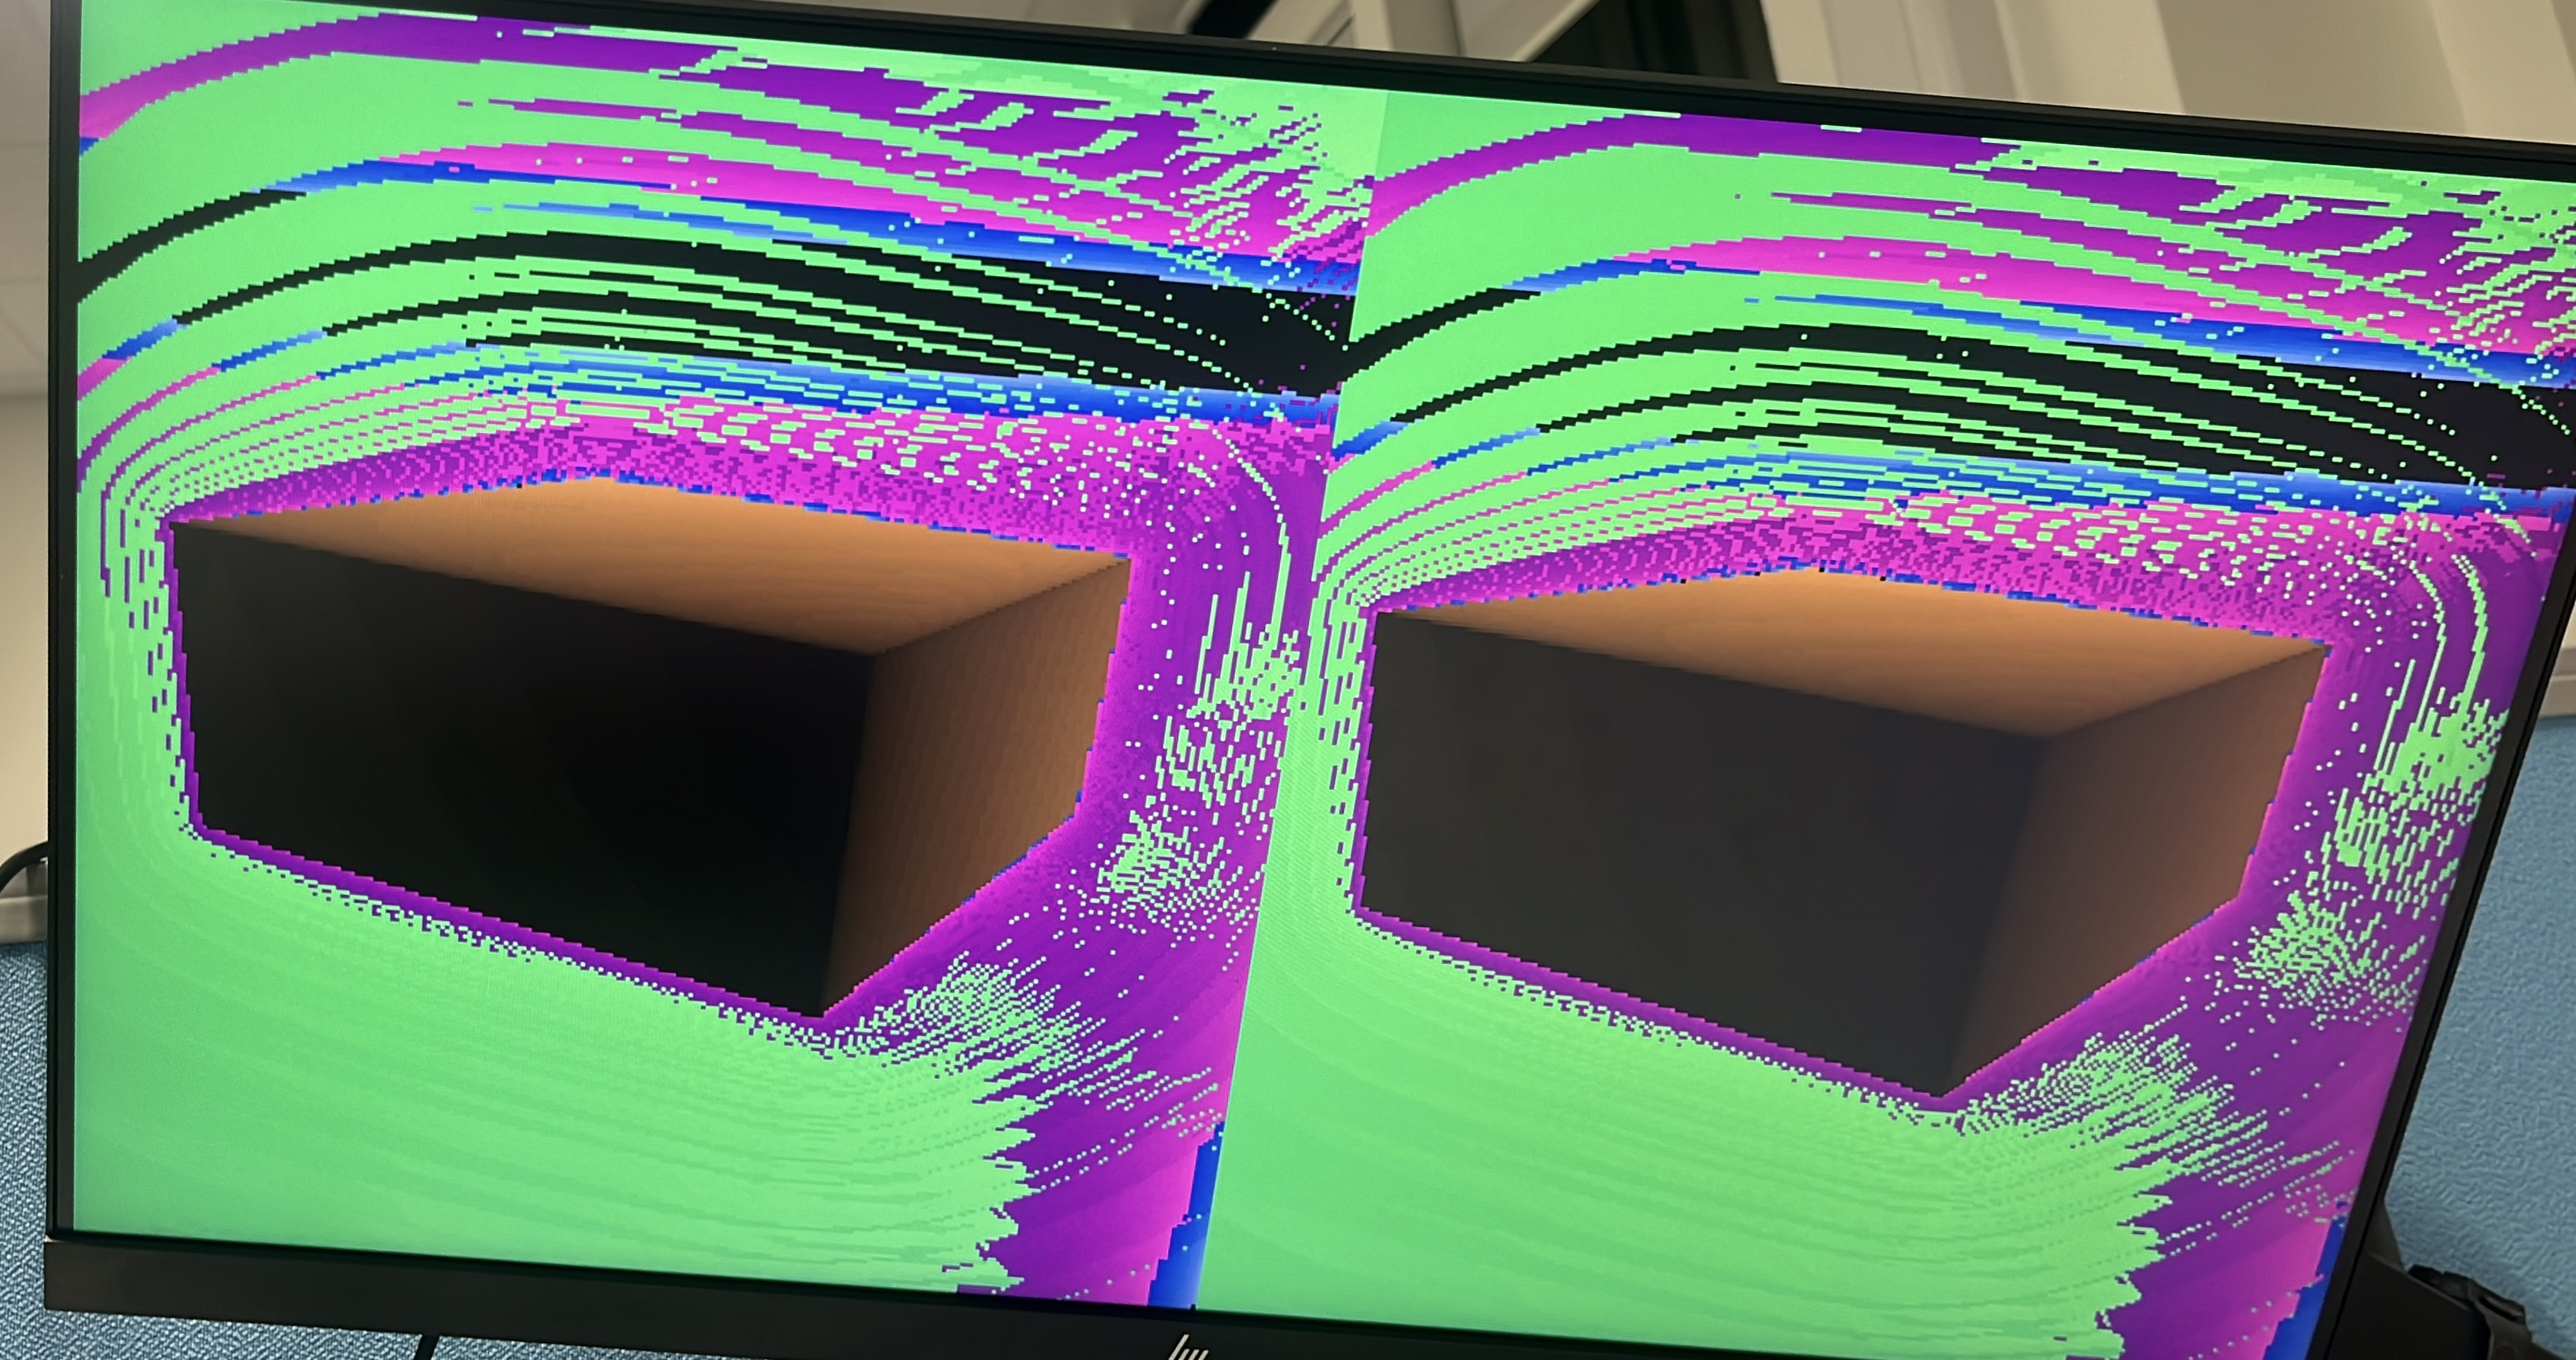
\includegraphics[width=\textwidth]{imgs/box_no_infinite.JPG}
        \vspace{-0.1cm} % Tighter padding between image and text
        \captionof{figure}{Initial renders of the box SDF, without space repetition. Notice the repeating colors in world borders due to palette.sv cyclical nature. 33 frames per second.}
        \label{fig:your_label}
    \end{minipage}
\end{center}